\documentclass{article}
\usepackage[utf8]{inputenc}
\usepackage{listings}
\usepackage{enumerate}
\usepackage{enumitem}
\title{DBcw2}
\author{dequn.teng }
\date{November 2019}
\usepackage{tikz}
\usepackage{natbib}
\usepackage{graphicx}
\usepackage{amsmath}
\usepackage{qtree}
\usepackage{float}
\begin{document}

\maketitle

\section{Question 1}
\begin{enumerate}[label=(\alph*)]
\item $\pi_{hotelName, city}(\sigma_{price > \pounds85 }(Hotel \times Room))$
\item $\pi_{guestName, guestAddress}(\sigma_{dateFrom\le `2019-12-25'\:AND\:dateTo \ge `2019-12-25'}(Booking \bowtie Guest))$

\end{enumerate}
\section{Question 2}
\begin{enumerate}[label=(\alph*)]
\item $\pi_{pId,owner,location}(\sigma_{sqrFeet>900}(property))$
\item $\pi_{company}(\sigma_{location=`Hyde Park'}(property\bowtie repairs))$


\end{enumerate}
\section{Question 3}
\begin{enumerate}[label=(\alph*)]
\item 200000(200000*40*50/2000). Answer: it needs 200000 blocks to store.
\item $\pi_{F\rule{0.1cm}{0.15mm}Name,L\rule{0.1cm}{0.15mm}Name,P\rule{0.1cm}{0.15mm}Name}( \sigma_{S.Prog\rule{0.1cm}{0.15mm}Code=`0001’}(S \bowtie P))	$

\item  
\begin{verbatim}
Select studId,lName
From STUDENT
Where course=’BSc’;
\end{verbatim}
\item 
\begin{verbatim}
Select Student.studno,Student.name
From Student,  Course 
Where Student.courseNo = Course.courseNo, AND Course.courseDep = `Comp Sci' 
AND Student.type ='undergrad' 
\end{verbatim}
\end{enumerate}


\section{Question 4}
\begin{enumerate}[label=(\alph*)]
\item 
Initial query plan is as follows.
\begin{center}
\begin{tikzpicture}[scale=0.2]
\tikzstyle{every node}+=[inner sep=0pt]

\draw (35.6,-11.4) node {$\pi_{B,E,G}$};

\draw (35.6,-20.7) node {$\sigma_{A=10\mbox{ }AND\mbox{ }E=F\mbox{ }AND\mbox{ }A>G}$};

\draw (35.6,-29.8) node {$\times$};

\draw (29.5,-37.3) node {$\times$};
\draw [black] (22.3,-45.5) circle (3);
\draw (22.3,-45.5) node {$R$};
\draw [black] (33.1,-45.5) circle (3);
\draw (33.1,-45.5) node {$S$};
\draw [black] (42.5,-37.3) circle (3);
\draw (42.5,-37.3) node {$T$};
\draw [black] (35.6,-14.4) -- (35.6,-17.7);
\fill [black] (35.6,-17.7) -- (36.1,-16.9) -- (35.1,-16.9);
\draw [black] (35.6,-23.7) -- (35.6,-26.8);
\fill [black] (35.6,-26.8) -- (36.1,-26) -- (35.1,-26);
\draw [black] (33.71,-32.13) -- (31.39,-34.97);
\fill [black] (31.39,-34.97) -- (32.29,-34.67) -- (31.51,-34.04);
\draw [black] (37.63,-32.01) -- (40.47,-35.09);
\fill [black] (40.47,-35.09) -- (40.3,-34.16) -- (39.56,-34.84);
\draw [black] (27.52,-39.55) -- (24.28,-43.25);
\fill [black] (24.28,-43.25) -- (25.18,-42.97) -- (24.43,-42.31);
\draw [black] (30.71,-40.05) -- (31.89,-42.75);
\fill [black] (31.89,-42.75) -- (32.03,-41.82) -- (31.11,-42.22);
\end{tikzpicture}
\end{center}

After pushing the selecting heuristic to the bottom, we get.
\begin{center}
\begin{tikzpicture}[scale=0.2]
\tikzstyle{every node}+=[inner sep=0pt]

\draw (35.6,-11.4) node {$\pi_{B,E,G}$};

\draw (35.6,-20.7) node {$\sigma_{E=F\mbox{ }AND\mbox{ }10>G}$};

\draw (35.6,-29.8) node {$\times$};

\draw (29.5,-37.3) node {$\times$};
\draw [black] (22.3,-45.5) circle (3);
\draw (22.3,-45.5) node {$R$};
\draw [black] (33.1,-45.5) circle (3);
\draw (33.1,-45.5) node {$S$};
\draw [black] (42.5,-37.3) circle (3);
\draw (42.5,-37.3) node {$T$};
\draw [black] (35.6,-14.4) -- (35.6,-17.7);
\fill [black] (35.6,-17.7) -- (36.1,-16.9) -- (35.1,-16.9);
\draw [black] (35.6,-23.7) -- (35.6,-26.8);
\fill [black] (35.6,-26.8) -- (36.1,-26) -- (35.1,-26);
\draw [black] (33.71,-32.13) -- (31.39,-34.97);
\fill [black] (31.39,-34.97) -- (32.29,-34.67) -- (31.51,-34.04);
\draw [black] (37.63,-32.01) -- (40.47,-35.09);
\fill [black] (40.47,-35.09) -- (40.3,-34.16) -- (39.56,-34.84);
\draw [black] (27.52,-39.55) -- (24.28,-43.25);
\fill [black] (24.28,-43.25) -- (25.18,-42.97) -- (24.43,-42.31);
\draw (25.36,-39.95) node [left] {$\sigma_{A=10}$};
\draw [black] (30.71,-40.05) -- (31.89,-42.75);
\fill [black] (31.89,-42.75) -- (32.03,-41.82) -- (31.11,-42.22);
\end{tikzpicture}
\end{center}
	introduce	equijoins	for	$\times$ followed	by	$\bowtie$, we get
\begin{center}
\begin{tikzpicture}[scale=0.2]
\tikzstyle{every node}+=[inner sep=0pt]

\draw (28.9,-18.8) node {$\bowtie_{E=F}$};

\draw (28.9,-7.1) node {$\pi_{B,E,G}$};
\draw [black] (34.8,-26.2) circle (3);
\draw (34.8,-26.2) node {$T$};

\draw (22,-27.2) node {$\bowtie_{C=D}$};

\draw (16.7,-34.4) node {$\sigma_{A=10}$};
\draw [black] (25.6,-35.1) circle (3);
\draw (25.6,-35.1) node {$S$};
\draw [black] (11.1,-42.7) circle (3);
\draw (11.1,-42.7) node {$R$};
\draw [black] (28.9,-10.1) -- (28.9,-15.8);
\fill [black] (28.9,-15.8) -- (29.4,-15) -- (28.4,-15);
\draw (28.4,-12.95) node [left] {$\sigma_{A>G}$};
\draw [black] (27,-21.12) -- (23.9,-24.88);
\fill [black] (23.9,-24.88) -- (24.8,-24.58) -- (24.03,-23.95);
\draw [black] (30.77,-21.15) -- (32.93,-23.85);
\fill [black] (32.93,-23.85) -- (32.82,-22.92) -- (32.04,-23.54);
\draw [black] (20.22,-29.62) -- (18.48,-31.98);
\fill [black] (18.48,-31.98) -- (19.36,-31.64) -- (18.55,-31.04);
\draw [black] (23.24,-29.93) -- (24.36,-32.37);
\fill [black] (24.36,-32.37) -- (24.48,-31.43) -- (23.57,-31.85);
\draw [black] (15.02,-36.89) -- (12.78,-40.21);
\fill [black] (12.78,-40.21) -- (13.64,-39.83) -- (12.81,-39.27);
\end{tikzpicture}
\end{center}
Finally, through pushing the selecting down, we get.
\begin{center}
\begin{tikzpicture}[scale=0.2]
\tikzstyle{every node}+=[inner sep=0pt]

\draw (28.9,-18.8) node {$\bowtie_{E=F}$};

\draw (28.9,-7.1) node {$\pi_{B,E,G}$};

\draw (33.6,-26.3) node {$\sigma_{10>G}$};

\draw (22,-27.2) node {$\bowtie_{C=D}$};

\draw (16.7,-34.4) node {$\sigma_{A=10}$};
\draw [black] (25.6,-35.1) circle (3);
\draw (25.6,-35.1) node {$S$};
\draw [black] (11.1,-42.7) circle (3);
\draw (11.1,-42.7) node {$R$};
\draw [black] (38.3,-33.8) circle (3);
\draw (38.3,-33.8) node {$T$};
\draw [black] (28.9,-10.1) -- (28.9,-15.8);
\fill [black] (28.9,-15.8) -- (29.4,-15) -- (28.4,-15);
\draw [black] (27,-21.12) -- (23.9,-24.88);
\fill [black] (23.9,-24.88) -- (24.8,-24.58) -- (24.03,-23.95);
\draw [black] (30.49,-21.34) -- (32.01,-23.76);
\fill [black] (32.01,-23.76) -- (32.01,-22.81) -- (31.16,-23.35);
\draw [black] (20.22,-29.62) -- (18.48,-31.98);
\fill [black] (18.48,-31.98) -- (19.36,-31.64) -- (18.55,-31.04);
\draw [black] (23.24,-29.93) -- (24.36,-32.37);
\fill [black] (24.36,-32.37) -- (24.48,-31.43) -- (23.57,-31.85);
\draw [black] (15.02,-36.89) -- (12.78,-40.21);
\fill [black] (12.78,-40.21) -- (13.64,-39.83) -- (12.81,-39.27);
\draw [black] (35.19,-28.84) -- (36.71,-31.26);
\fill [black] (36.71,-31.26) -- (36.71,-30.31) -- (35.86,-30.85);
\end{tikzpicture}
\end{center}
Finally, we put the projection to the bottom
\begin{center}
\begin{tikzpicture}[scale=0.2]
\tikzstyle{every node}+=[inner sep=0pt]

\draw (28.9,-18.8) node {$\bowtie_{E=F}$};

\draw (28.9,-7.1) node {$\pi_{B,E,G}$};

\draw (33.6,-26.3) node {$\sigma_{10>G}$};

\draw (15.8,-33.8) node {$\bowtie_{C=D}$};

\draw (5.2,-48) node {$\sigma_{A=10}$};
\draw [black] (21.8,-41.5) circle (3);
\draw (21.8,-41.5) node {$S$};
\draw [black] (5.2,-56) circle (3);
\draw (5.2,-56) node {$R$};
\draw [black] (38.3,-33.8) circle (3);
\draw (38.3,-33.8) node {$T$};

\draw (21.8,-26.3) node {$\pi_{B,E}$};

\draw (9.8,-40) node {$\pi_{B,C}$};
\draw [black] (28.9,-10.1) -- (28.9,-15.8);
\fill [black] (28.9,-15.8) -- (29.4,-15) -- (28.4,-15);
\draw [black] (30.49,-21.34) -- (32.01,-23.76);
\fill [black] (32.01,-23.76) -- (32.01,-22.81) -- (31.16,-23.35);
\draw [black] (17.64,-36.17) -- (19.96,-39.13);
\fill [black] (19.96,-39.13) -- (19.86,-38.2) -- (19.07,-38.81);
\draw [black] (5.2,-51) -- (5.2,-53);
\fill [black] (5.2,-53) -- (5.7,-52.2) -- (4.7,-52.2);
\draw [black] (35.19,-28.84) -- (36.71,-31.26);
\fill [black] (36.71,-31.26) -- (36.71,-30.31) -- (35.86,-30.85);
\draw [black] (26.84,-20.98) -- (23.86,-24.12);
\fill [black] (23.86,-24.12) -- (24.78,-23.88) -- (24.05,-23.2);
\draw [black] (19.93,-28.64) -- (17.67,-31.46);
\fill [black] (17.67,-31.46) -- (18.56,-31.15) -- (17.78,-30.52);
\draw [black] (13.71,-35.96) -- (11.89,-37.84);
\fill [black] (11.89,-37.84) -- (12.8,-37.62) -- (12.08,-36.92);
\draw [black] (8.3,-42.6) -- (6.7,-45.4);
\fill [black] (6.7,-45.4) -- (7.53,-44.95) -- (6.66,-44.46);
\end{tikzpicture}
\end{center}

\item 
In this question, we assume the value within the relationship is evenly distributed.

1) Since the number of tuples regarding to A in R is 1000, and the number of distinct values in R is 1000. Therefore, the number of tuple returned is 1.
\begin{equation}
    =\frac{\# tuples}{\# distinct values}=\frac{1000}{1000}=1
\end{equation}
2)
There are two scenarios in this case, where A is 1 and B is b at the same time, and A is 1 and B is b are not happening at the same time. 

In the first case, the number of distinct values of A in R plus the number of distinct values of B in R minus 1.
\begin{equation}
    =\frac{\#tuples}{\# of distinct\,A\,of\,R}+\frac{\# tuples}{\# of distinct\,B\,of\,R}-1=1+\frac{1000}{100}-1=10
\end{equation}

In the second case, the number of distinct values of A in R, plus the number of distinct values in B in R.
\begin{equation}
      =\frac{\#tuples}{\# of distinct\,A\,of\,R}+\frac{\# tuples}{\# of distinct\,B\,of\,R}=1+\frac{1000}{100}=11
\end{equation}
3)
Since it is an equal join, it is equal to the number of tuples in R times the number of tuples in S, divided by the maximum number of distinct values for A in R or S
\begin{equation}
    \frac{\mid R \mid \times \mid S \mid }{max(distinct\,values\,for\,A\,in\,R\,or\,S)}=\frac{1000*5000}{500}=10000
\end{equation}
\item  
 $$\sigma_{B=b AND E=100}(R \bowtie_{C=D}S)$$
 This query is based on a join query.
According to CMU database group, the quickest join algorithm is hash join, illustrated in the following figure \ref{fig:my_label} \cite{CMU1544518:online}.
\begin{figure}[H]
    \centering
    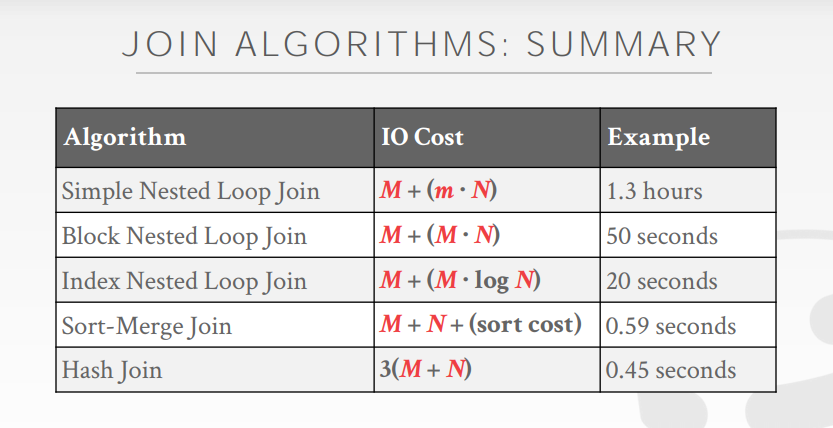
\includegraphics[width=14cm]{Capture.PNG}
    \caption{Join algorithm comparison}
    \label{fig:my_label}
\end{figure}
However, since the hash join use the index system, which is not allowed in this question. Therefore, we use the sort-merge join algorithm to do be the fastest query plan in this question. 

Based on the slice notation, we assume M to be the number of disk block fit into RAM.
B=10, since one block can only hold 10 tuples.
The number of disk operation is equal to the number of times going into the block.

In order to figure out the number of disk operations, the query can be representation as the following tree structure.
\begin{center}
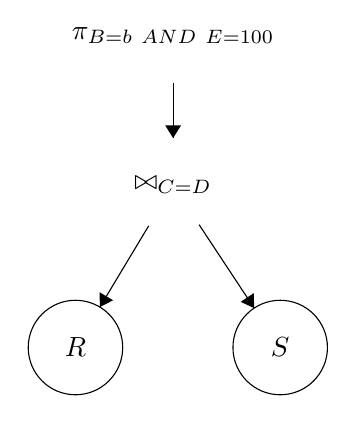
\begin{tikzpicture}[scale=0.2]
\tikzstyle{every node}+=[inner sep=0pt]

\draw (28,-8.6) node {$\pi_{B=b\mbox{ }AND\mbox{ }E=100}$};

\draw (28,-18.1) node {$\bowtie_{C=D}$};
\draw [black] (21.8,-28.4) circle (3);
\draw (21.8,-28.4) node {$R$};
\draw [black] (34.8,-28.4) circle (3);
\draw (34.8,-28.4) node {$S$};
\draw [black] (28,-11.6) -- (28,-15.1);
\fill [black] (28,-15.1) -- (28.5,-14.3) -- (27.5,-14.3);
\draw [black] (26.45,-20.67) -- (23.35,-25.83);
\fill [black] (23.35,-25.83) -- (24.19,-25.4) -- (23.33,-24.89);
\draw [black] (29.65,-20.6) -- (33.15,-25.9);
\fill [black] (33.15,-25.9) -- (33.12,-24.95) -- (32.29,-25.5);
\end{tikzpicture}
\end{center}
The quicker version is as follows through using heuristics.
\begin{center}
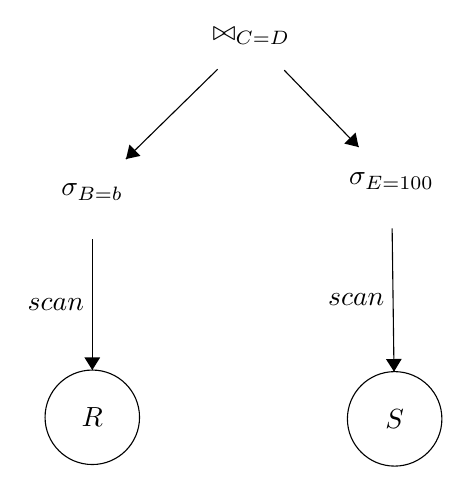
\begin{tikzpicture}[scale=0.2]
\tikzstyle{every node}+=[inner sep=0pt]

\draw (22.7,-14.3) node {$\bowtie_{C=D}$};

\draw (12.6,-24.2) node {$\sigma_{B=b}$};

\draw (31.6,-23.5) node {$\sigma_{E=100}$};
\draw [black] (12.6,-38.5) circle (3);
\draw (12.6,-38.5) node {$R$};
\draw [black] (31.8,-38.6) circle (3);
\draw (31.8,-38.6) node {$S$};
\draw [black] (20.56,-16.4) -- (14.74,-22.1);
\fill [black] (14.74,-22.1) -- (15.66,-21.9) -- (14.96,-21.18);
\draw [black] (24.79,-16.46) -- (29.51,-21.34);
\fill [black] (29.51,-21.34) -- (29.32,-20.42) -- (28.6,-21.12);
\draw [black] (12.6,-27.2) -- (12.6,-35.5);
\fill [black] (12.6,-35.5) -- (13.1,-34.7) -- (12.1,-34.7);
\draw (12.1,-31.35) node [left] {$scan$};
\draw [black] (31.64,-26.5) -- (31.76,-35.6);
\fill [black] (31.76,-35.6) -- (32.25,-34.79) -- (31.25,-34.81);
\draw (31.18,-31.05) node [left] {$scan$};
\end{tikzpicture}
\end{center}
After that, we should evaluate these information part by part. 

The first part is select B=b in relationship R. It will take $\frac{\mid R \mid }{10}$ disk operations, since it scan through the disk. Let R' to be the table only contain B=b, it contains 10 tuples assuming values of B is evenly distributed.

The second part is select E=100 in relationship S. It will take $\frac{\mid S \mid }{10}$ disk operations, since it scan through the disk. Let S' to be the table only contain tuples where E=100. There are $\frac{5000}{10}$,   which is 500 tuples in S'.


The third part is the equal join using C=D on S' and R'. The join algorithm used here is Sort Join	Algorithm (Figure \ref{fig:my_label2}) \cite{Chapter329:online}. 
\begin{figure}[H]
    \centering
    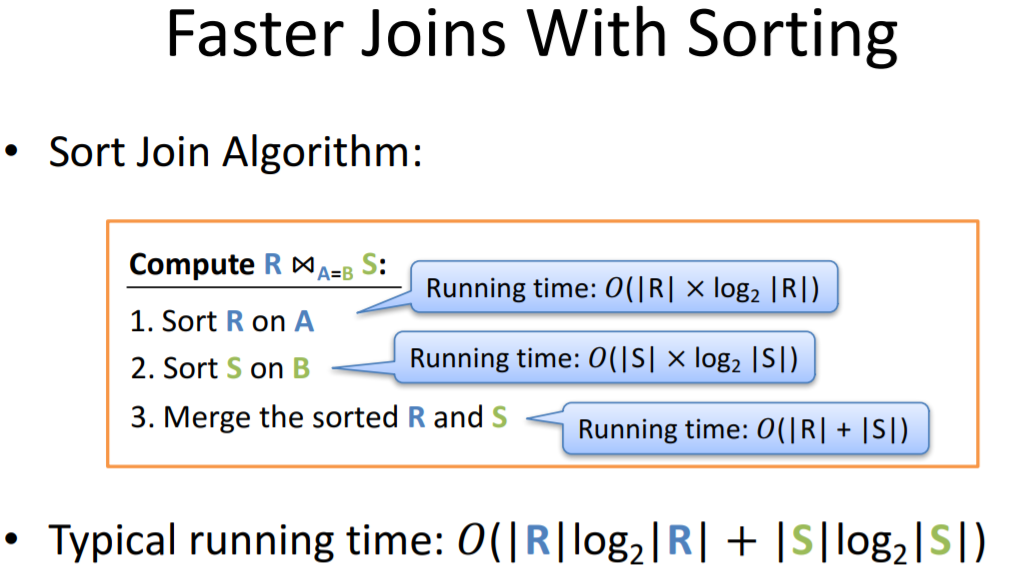
\includegraphics[width=14cm]{6.png}
    \caption{Sort Join Algorithm}
    \label{fig:my_label2}
\end{figure}
Sort R' on C will take $O(\frac{\mid R' \mid}{10}\times \log_2 \frac{\mid R' \mid}{10} ) $ disk operations. (Result is 0 disk operation).

Sort S' on C will take $O( \frac{\mid S' \mid}{10} \times \log_2\frac{\mid S' \mid}{10}  ) $ disk operations. (Result is 283, to the ceiling)

Merge the sorted R' and S', will take $O(\frac{\mid R \mid +\mid S \mid }{10})$, which is 51 times of disk operation. 

\begin{multline}
     \# operations=\frac{\mid R \mid}{10}+\frac{\mid S \mid}{10}+O(\frac{\mid R' \mid}{10}\times \log_2 \frac{\mid R' \mid}{10} )+\\O( \frac{\mid S' \mid}{10} \times \log_2\frac{\mid S' \mid}{10}  )+O(\frac{\mid R' \mid +\mid S' \mid }{10})
\end{multline}

   

The final answer is 
\begin{equation}
    =100+500+0+282+51=933
\end{equation}
Since it is a big O notation, we can ignore the $O(\frac{\mid R' \mid +\mid S'\mid }{10}$, we have 882 disk opertions.


\bibliographystyle{plain}
\bibliography{references}
\end{enumerate}
\end{document}

